\section{Linkages}
\begin{figure}[!htbp]
 \begin{center}
  \includegraphics{graphics/HumanTurkeyLinkage.pdf}
  \caption{Here are skeleton drawings of a human and a turkey.  When animating skeletons, one tends to make sure that the lengths of the skeleton segments are kept the same length throught the animation.  Otherwise, the animation may depart from what is ideally understood of skeletal motions.}
 \end{center} 
\end{figure}

When graph drawings model physical objects, other qualities about the graph can be contextualized in a geometric sense.  
Distance, angular relationstips and other geometric qualities of the drawings can be other useful properties of the drawing to perform analysis on.
The \textit{length assignment} of a graph $G=(V,E)$ is $\ell:E \mapsto \bbr^+$. 
For simple graphs, length assignment must be strictly positive, otherwise it may result in two distinct vertices with the same coordinates.
A \textit{linkage} is a graph $G = (V,E)$ with a length assignment $\ell:E \mapsto \bbr^+$.  
Length assignments can be thought of as a metric where $\ell(u,v) = \ell(v,u)>0$.
%Inser linkage here




% \begin{figure}[!h]
% \begin{center}
% 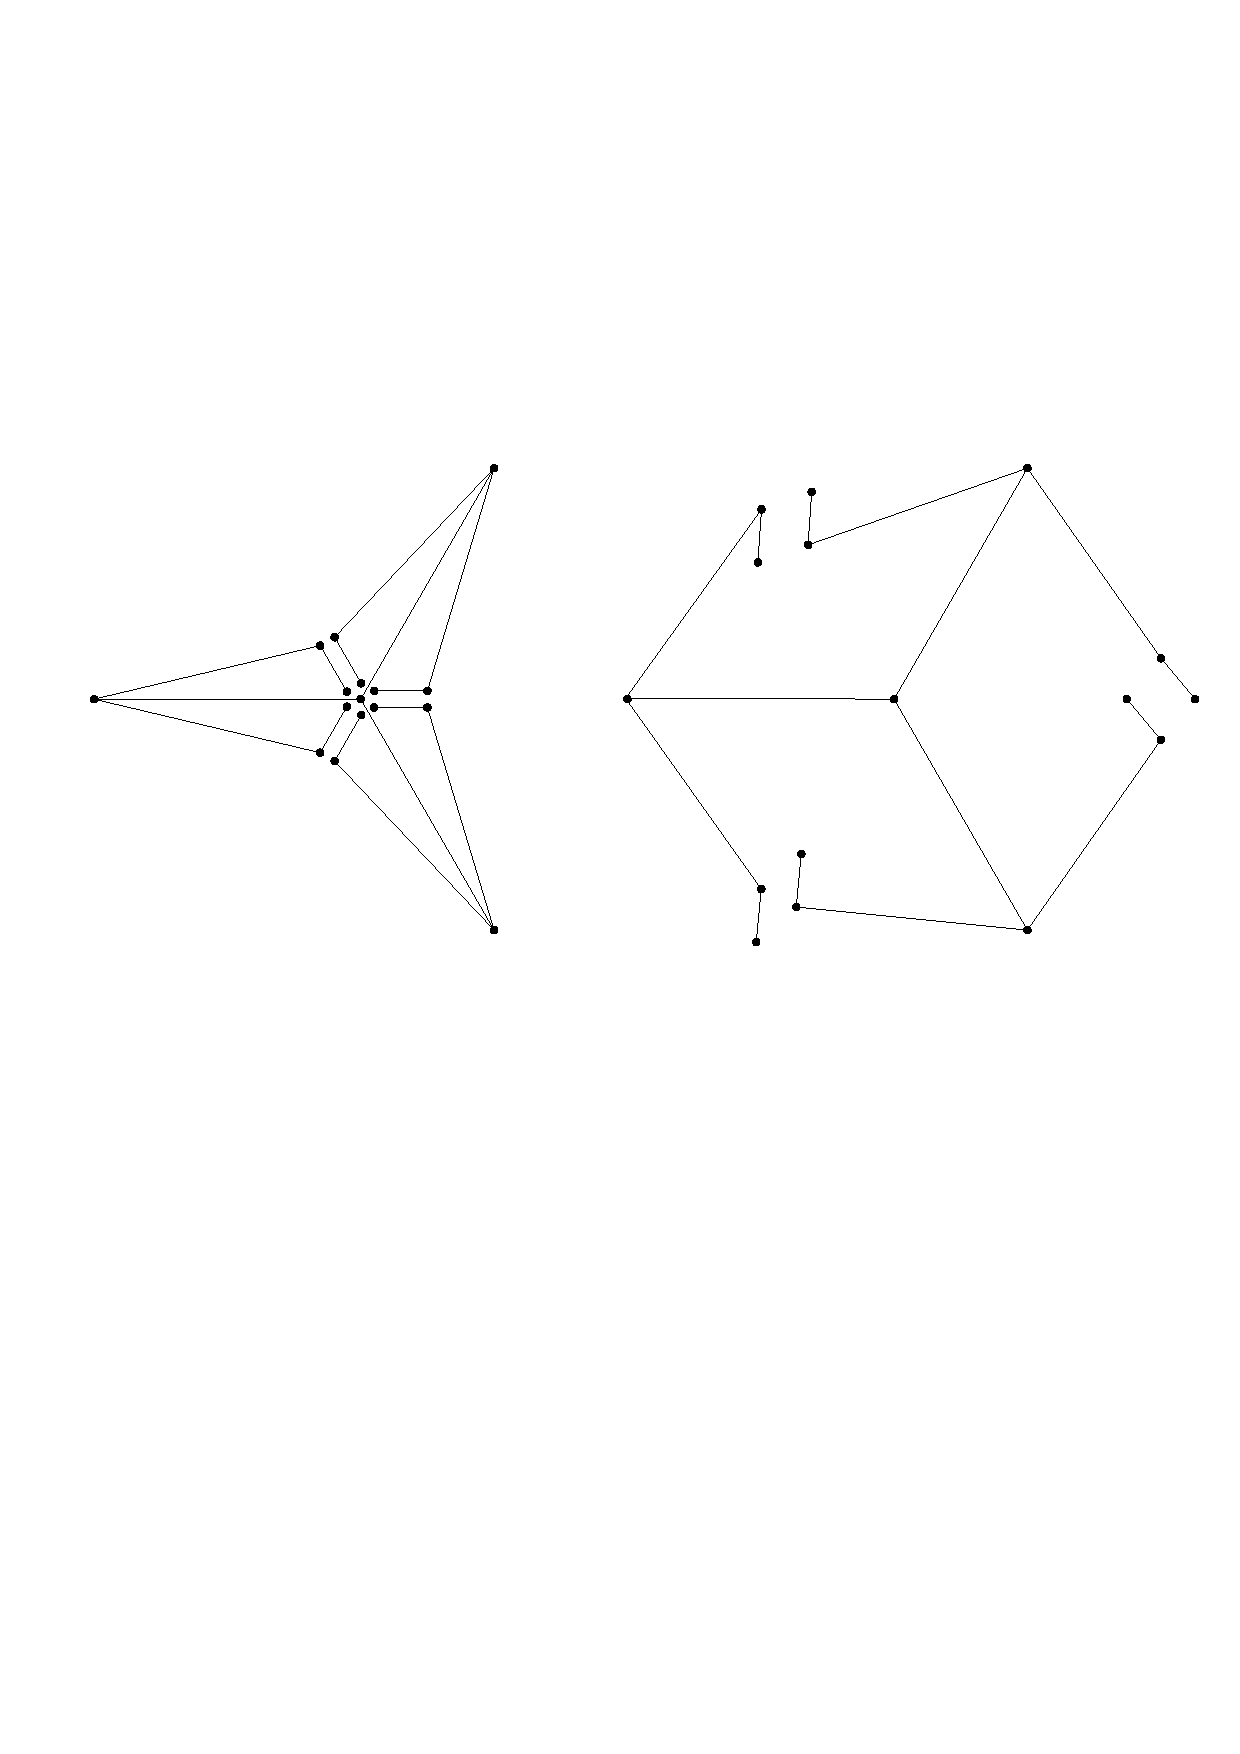
\includegraphics[scale=.75]{graphics/LockedConnellyLinkage.pdf}
% \end{center} 
% \caption{A linkage whose complete configuration space is discontinuous.  These two examples above 
% are two configurations of the same linkage that cannot continuously transform into the other 
% without edge crossing.}
% \label{fig:configuration-4}
% \end{figure}
% A \textit{reconfiguration} of a linkage whose graph is $G=(V,E)$ and length assignment is $\ell$ is 
% a continuous function $f: [0,1] \mapsto \bbr^{2 \cdot \vert V \vert}$ specifying a configuration of 
% the linkage for every $t \in [0,1]$ where length assignment $\ell$ is preserved, edges do not cross 
% and for every $\epsilon > 0$, there exists a $\delta > 0$ such that $\vert t_1 - t_2 \vert < 
% \delta$ implies 
% $$\left\vert f\left( t_1 \right) - f\left( t_2 \right) \right\vert < \epsilon$$

%(fig 1) insert a table of a graph and define a length assigment 
%(fig 2) insert a realization of (fig 1)
%(fig 3) insert a second realization of (fig 1)



%graph component of the linkage   the plane.  A linkage 
%\textit{embedding} is $L : V \mapsto 
%\bbR^{2}$.
% A \textit{linkage} is an ordered pair $G = (V,E)$ comprising of a set $V$ of vertices or nodes 
% together with a set $E$ of edges or lines. This definition is commonly used for graphs.  Mapping 
% the linkage $G$ into the plane is said to be the \textit{embedding}, i.e. $L : V \mapsto 
% \bbR^{2}$.  A length function correspond to a linkage, $l: E \mapsto \bbr^+$ gives a length to an 
% edge in the linkage.  If We consider a \textit{realization} of a linkage is range of $L$, i.e. 
% $L(V)$. If for every edge $(u,v) \in E$ such that $l\left( \left(u,v\right) \right) = \left\vert 
% L(u) - L(v) \right\vert$ is true, then $L$ is said to be a \textit{proper embedding} of $G$.
% \begin{figure}[h]
% \begin{center}
% 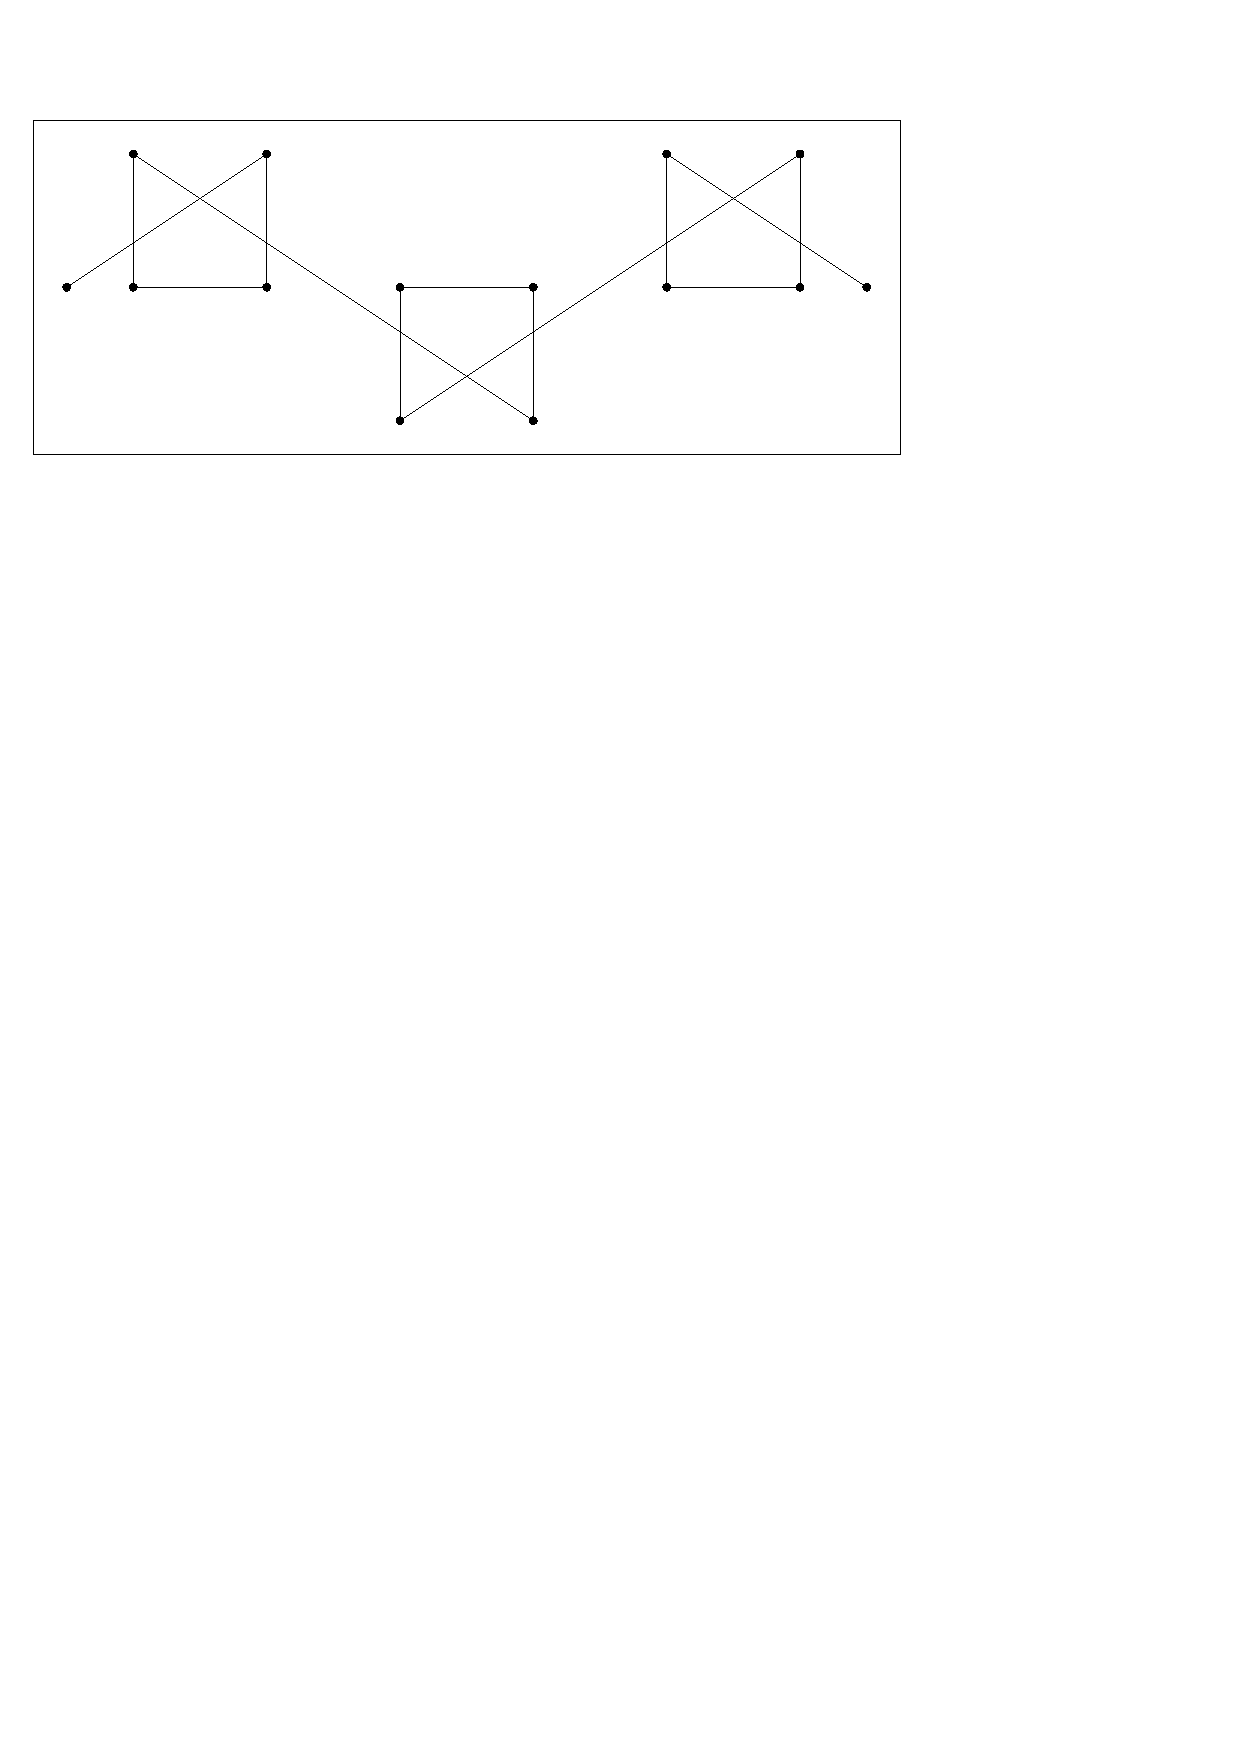
\includegraphics[scale=1]{graphics/crossingEdgeLinkage.pdf}
% \end{center} 
% \caption{A linkage where edges cross however it does not contain loops or multiple edges between 
% vertices.}
% \label{fig:linkage-3}
% \end{figure}
